% Tikz File 'AMR.tex'
\documentclass{standalone}
\usepackage{tikz}
\usetikzlibrary {arrows.meta} 
\begin{document}
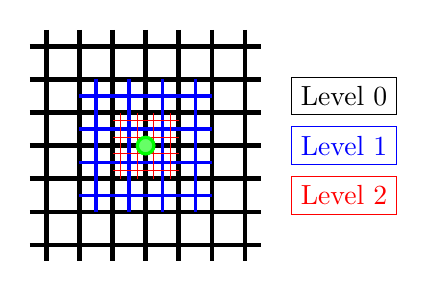
\begin{tikzpicture}[scale=0.21]
	\draw[ultra thick] (6,7) -- (6,-7);
	\draw[ultra thick] (4,7) -- (4,-7);
	\draw[ultra thick] (2,7) -- (2,-7);
	\draw[ultra thick] (0,7) -- (0,-7);
	\draw[ultra thick] (-2,7) -- (-2,-7);
	\draw[ultra thick] (-4,7) -- (-4,-7);
	\draw[ultra thick] (-6,7) -- (-6,-7);
	\draw[ultra thick] (-7,6) -- (7,6);
	\draw[ultra thick] (-7,4) -- (7,4);
	\draw[ultra thick] (-7,2) -- (7,2);
	\draw[ultra thick] (-7,0) -- (7,0);
	\draw[ultra thick] (-7,-2) -- (7,-2);
	\draw[ultra thick] (-7,-4) -- (7,-4);
	\draw[ultra thick] (-7,-6) -- (7,-6);
	\draw[blue, very thick] (1,4) -- (1,-4);
	\draw[blue, very thick] (-1,4) -- (-1,-4);
	\draw[blue, very thick] (3,4) -- (3,-4);
	\draw[blue, very thick] (-3,4) -- (-3,-4);
	\draw[blue, very thick] (-4,1) -- (4,1);
	\draw[blue, very thick] (-4,-1) -- (4,-1);
	\draw[blue, very thick] (-4,3) -- (4,3);
	\draw[blue, very thick] (-4,-3) -- (4,-3);

	\draw[red] (-1.5,-2) -- (-1.5,2);
	\draw[red] (-0.5,-2) -- (-0.5,2);
	\draw[red] (0.5,-2) -- (0.5,2);
	\draw[red] (1.5,-2) -- (1.5,2);
	\draw[red] (-2,-1.5) -- (2,-1.5);
	\draw[red] (-2,-0.5) -- (2,-0.5);
	\draw[red] (-2,0.5) -- (2,0.5);
	\draw[red] (-2,1.5) -- (2,1.5);
	\filldraw[color=green, fill=green!60, very thick](0,0) circle (0.5);
	\node[draw,black] at (12,3) {Level 0};
	\node[draw,blue] at (12,0) {Level 1};
	\node[draw,red] at (12,-3) {Level 2};
\end{tikzpicture}
\end{document}